\documentclass[11pt, a4paper]{article}
\usepackage{polski}
\usepackage[utf8]{inputenc}
\usepackage[T1]{fontenc}
\usepackage[export]{adjustbox}
\usepackage{graphicx}
\usepackage{amsmath} 
\usepackage{listings}
\usepackage{color}
\usepackage{marvosym}
\usepackage{geometry}
\usepackage{float}
\usepackage{booktabs}
\usepackage{multirow}
\usepackage{titlesec}
\usepackage{hyperref}
\usepackage{tabularx}

\geometry{margin=1.2in}
\usepackage[final]{pdfpages}

\newcommand{\fbi}{\leavevmode{\parindent=1em\indent}}

\definecolor{dkgreen}{rgb}{0,0.6,0}
\definecolor{gray}{rgb}{0.5,0.5,0.5}
\definecolor{mauve}{rgb}{0.58,0,0.82}

\lstset{
	frame=tblr,
	language=R,
	aboveskip=3mm,
	belowskip=3mm,
	showstringspaces=false,
	columns=flexible,
	basicstyle={\small\ttfamily},
	numbers=left,
	numberstyle=\tiny\color{gray},
	keywordstyle=\color{blue},
	commentstyle=\color{dkgreen},
	stringstyle=\color{mauve},
	breaklines=true,
	mathescape=false,
	breakatwhitespace=true,
	tabsize=3,
	inputencoding=utf8,
	extendedchars=true,
	literate=
	{ą}{{\k{a}}}1
	{Ą}{{\k{A}}}1
	{ę}{{\k{e}}}1
	{Ę}{{\k{E}}}1
	{ó}{{\'o}}1
	{Ó}{{\'O}}1
	{ś}{{\'s}}1
	{Ś}{{\'S}}1
	{ł}{{\l{}}}1
	{Ł}{{\L{}}}1
	{ż}{{\.z}}1
	{Ż}{{\.Z}}1
	{ź}{{\'z}}1
	{Ź}{{\'Z}}1
	{ć}{{\'c}}1
	{Ć}{{\'C}}1
	{ń}{{\'n}}1
	{Ń}{{\'N}}1
}

\renewcommand\lstlistingname{Listing}

\titleclass{\subsubsubsection}{straight}[\subsection]
\newcounter{subsubsubsection}[subsubsection]
\renewcommand\thesubsubsubsection{\thesubsubsection.\arabic{subsubsubsection}}
\renewcommand\theparagraph{\thesubsubsubsection.\arabic{paragraph}}

\titleformat{\subsubsubsection}
  {\normalfont\normalsize\bfseries}{\thesubsubsubsection}{1em}{}
\titlespacing*{\subsubsubsection}
{0pt}{3.25ex plus 1ex minus .2ex}{1.5ex plus .2ex}

\makeatletter
\renewcommand\paragraph{\@startsection{paragraph}{5}{\z@}
  {3.25ex \@plus1ex \@minus.2ex}
  {-0em}
  {\normalfont\normalsize\bfseries}}
\renewcommand\subparagraph{\@startsection{subparagraph}{6}{\parindent}
  {3.25ex \@plus1ex \@minus .2ex}
  {-1em}
  {\normalfont\normalsize\bfseries}}
\def\toclevel@subsubsubsection{4}
\def\toclevel@paragraph{5}
\def\toclevel@paragraph{6}
\def\l@subsubsubsection{\@dottedtocline{4}{7em}{4em}}
\def\l@paragraph{\@dottedtocline{5}{10em}{5em}}
\def\l@subparagraph{\@dottedtocline{6}{14em}{6em}}
\makeatother

\setcounter{secnumdepth}{4}
\setcounter{tocdepth}{4}

\hypersetup{pageanchor=false}

\setlength\parindent{3pt}

\renewcommand{\labelenumi}{\alph{enumi}.} 

\date{\today}

\begin{document}

\begin{titlepage}

\newcommand{\HRule}{\rule{\linewidth}{0.5mm}} 
\center 

\textsc{\LARGE Politechnika Wrocławska}\\[1.5cm] 
\textsc{\Large Inteligencja Obliczeniowa i jej zastosowania}\\[0.5cm] 
\HRule \\[0.5cm]
{ \huge \bfseries Badanie algorytmu genetycznego z zakresu optymalizacji globalnej dla wybranej funkcji testowej. Przeprowadzenie pomiarów dla algorytmu hybrydowego i optymalizacji rojem cząstek }\\[0.5cm] 
\HRule \\[1.6cm]
 
\begin{minipage}{0.4\textwidth}
\begin{flushleft} \large
\emph{Autorzy:}\\
Paweł  \textsc{Andziul} 200648 \\
Marcin  \textsc{Słowiński} 200638 \\
\end{flushleft}
\end{minipage}
~
\begin{minipage}{0.4\textwidth}
\begin{flushright} \large
\emph{Prowadzący:} \\
dr hab. inż. Olgierd \textsc{Unold}, prof. nadzw. PWr
\end{flushright}
\end{minipage}\\[4cm]

\vfill 
{\large 26 kwietnia 2017}\\[3cm] 

\end{titlepage}

\tableofcontents

\newpage
\section{Wprowadzenie}
\paragraph{}
Algorytm genetyczny jest algorytmem heurystycznym, który swoim działaniem przypomina działanie ewolucji w~naturze. Osobniki będące zbyt słabymi zostają wyeliminowane z~populacji w~kolejnych pokoleniach, a~na ich miejsce przyjmowane są lepsze, silniejsze, bardziej podatne adaptacji. Algorytm ten zakłada możliwość mutacji i~krzyżowania wśród potomków, przez co nie zawsze są oni silniejsi od poprzednio wyeliminowanych członków. Dodatkowo wprowadza się pojęcie elity, która jest bezpośrednio przenoszona do następnego - teoretycznie lepszego pokolenia.

\fbi
Algorytm memetyczny to hybrydowy algorytm ewolucyjny będący uzupełnieniem algorytmu genetycznego o dodatkowe, poza krzyżowaniem i mutacją, operatory tworzenia osobników kolejnej generacji.

\fbi
Algorytm PSO jest to natomiast algorytm optymalizacji rojem cząstek. Każda z cząstek z populacji (roju) jest umieszczana na losowej pozycji w przestrzeni rozwiązań. Pozycja każdej z cząstki podlega ocenie poprzez funkcję dopasowania. Z każdą cząstką związany jest dodatkowo pewien wektor prędkości z jaką się ona porusza. W każdej iteracji wektory odpowiadające pozycji cząstki oraz prędkości są sumowane. Na prędkość każdej z cząstek ma wpływ pozycja o największym dopasowaniu znaleziona przez cały rój oraz pozycja o największym dopasowaniu znaleziona przez konkretną cząstkę. Przebieg algorytmu dla przestrzeni 3-wymiarowej może być w interesujący sposób zwizualizowany.

\fbi
Problem komiwojażera - jest zagadnieniem optymalizacyjnym, w~którym optymalizowana jest długość trasy między miastami, tak by odnaleźć najkrótszą drogę nie omijając żadnego z nich. W części poświęconej temu problemowi zamieszczono szersze wyjaśnienie.

\fbi
W ramach laboratorium należało przeprowadzić testy algorytmów porównując działanie domyślnej i własnej funkcji mutacji (zarówno dla problemu optymalizacji rzeczywistej jak i TSP). Dodatkowo należało wykonać testy unikalnych parametrów algorytmu memetycznego i PSO.

\fbi
Pomiary wykonywano na 2 różnych jednostkach roboczych. Ich parametry nie są istotne z~punktu widzenia analizy i~możliwości porównania rezultatów.

\newpage
\section{Poblem optymalizacji rzeczywistej (funkcja Hartman6)}
\paragraph{}
Hartman6 jest funkcją określoną dla ilości parametrów równej 6. Na ilustracji (rys.~\ref{fig:Hartman6_overview}) przedstawiono jej wykres dla pierwszych dwóch. Poniżej zamieszczono jej wzór (\ref{eq:hartman6}).

\begin{equation}\label{eq:hartman6}
f(\boldsymbol{x}) = - \sum_{i=1}^{4} c_i \exp[- \sum_{j=1}^{6} a_{ij}(x_j - p_{ij})^2]
\end{equation}

, gdzie $ x_i \in [0, 1] $, $ i~\in \{1, ..., 6\} $.

\begin{figure}[H]
	\centering
	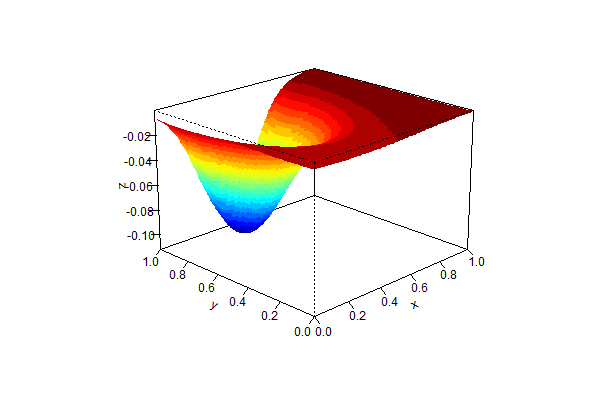
\includegraphics[width=0.95\textwidth]{./assets/Hartman6_overview.png}
	\caption{Wykres funkcji Hartman6}
	\label{fig:Hartman6_overview}
\end{figure}

\subsection{Badanie algorytmu genetycznego dla własnej funkcji mutacji}
\paragraph{}
Badania przeprowadzono dla algorytmu genetycznego w wersji podstawowej, ze zmienioną funkcją mutacji oraz hybrydowej, a także dla algorytmu optymalizacji rojem cząstek (PSO). W tym punkcie zamieszczono wyniki dotyczące wpływu własnej funkcji mutacji na poziom optymalizacji.

\fbi
Własna funkcja mutacji została utworzona w taki sposób by nie doprowadzić do sytuacji, w której przekroczona zostanie minimalna lub maksymalna wartość populacji. Jej działanie opiera się na wybraniu minimalnej jednostki z populacji i podmianie innej, losowej na znalezioną minimalną. Gwarantuje to niepojawienie się w populacji wartości uznawanej przez algorytm za niepoprawną.

\begin{figure}[H]
	\centering
	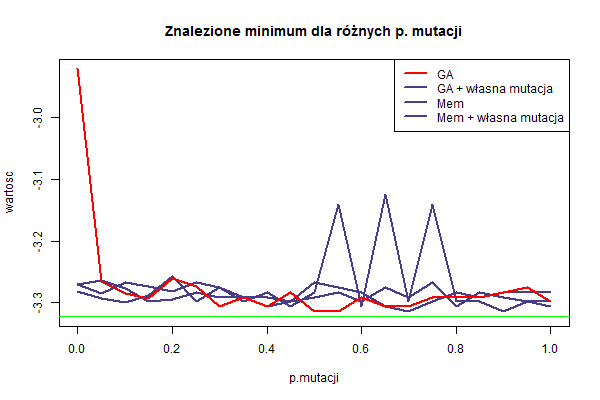
\includegraphics[width=0.95\textwidth]{./assets/Hartman6mut1.png}
	\caption{Wykres funkcji Hartman6}
	\label{fig:Hartman6mut1}
\end{figure}

\begin{figure}[H]
	\centering
	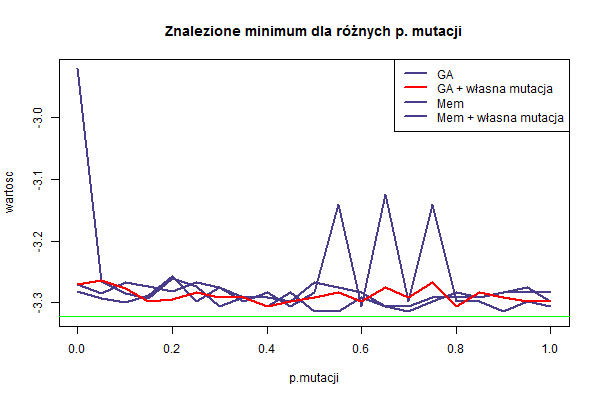
\includegraphics[width=0.95\textwidth]{./assets/Hartman6mut2.png}
	\caption{Wykres funkcji Hartman6}
	\label{fig:Hartman6mut2}
\end{figure}

\begin{figure}[H]
	\centering
	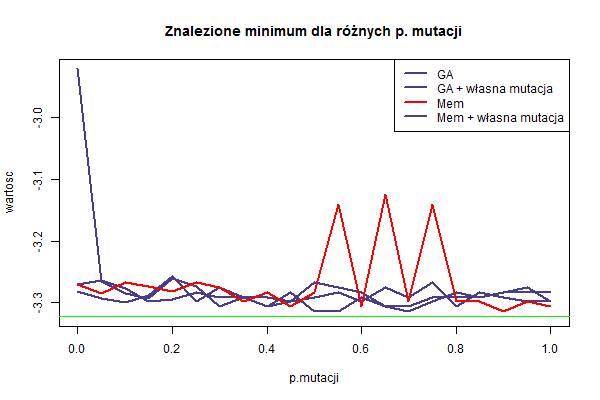
\includegraphics[width=0.95\textwidth]{./assets/Hartman6mut3.png}
	\caption{Wykres funkcji Hartman6}
	\label{fig:Hartman6mut3}
\end{figure}

\begin{figure}[H]
	\centering
	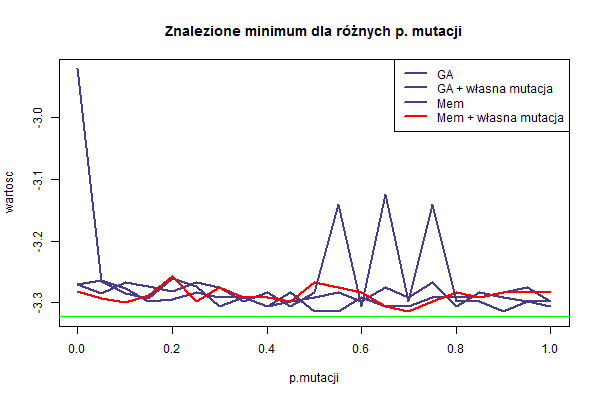
\includegraphics[width=0.95\textwidth]{./assets/Hartman6mut4.png}
	\caption{Wykres funkcji Hartman6}
	\label{fig:Hartman6mut4}
\end{figure}

\fbi
Z wykresów można odczytać zbliżone wyniki dla różnych funkcji mutacji. Żadna z~funkcji nie osiągnęła minimum co świadczy o tym, że sama mutacja tutaj nie jest wystarczająca. Zauważalny jest również niski wpływ własnej funkcji mutacji na otrzymywane wyniki. Pod względem jakości rozwiązań nie odstaje ona od istniejących implementacji. Na wykresach można zauważyć znaczące pogorszenie się wyników dla funkcji memetycznej z domyślną funkcją mutacji. W przedziale 0.5 -- 0.8 wygenerowała ona wyniki widocznie odstające od reszty.


\subsection{Badanie algorytmów dla różnych wartości ich unikalnych parametrów}
\paragraph{}
Algorytmy memetyczny i PSO posiadają własne wartości unikalne, których zmiana może wpłynąć na otrzymywane wyniki. Poniżej przedstawiono wykresy przedstawiające otrzymane wartości optimum przy zmianie wybranych parametrów. Badania przeprowadzono w przedziale 0 -- 1 z krokiem co 0,01. Otrzymane wyniki są uśrednione na podstawie 30 iteracji.

\begin{figure}[H]
	\centering
	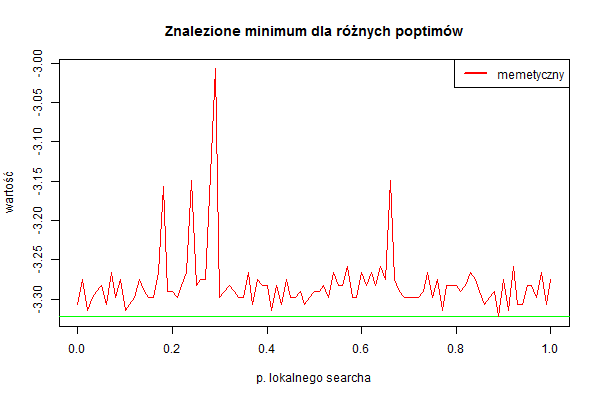
\includegraphics[width=0.95\textwidth]{./assets/Hartman6poptim.png}
	\caption{Jakość rozwiązań dla różnych wartości poptimum (memetyczny)}
	\label{fig:hybridpoptimum}
\end{figure}

\fbi
Z wykresu (rys.~\ref{fig:hybridpoptimum}) można odczytać niski wpływ wartości poptimum na otrzymane wyniki. Otrzymywane wartości różnią się nie więcej niż o 0,30. Przy czym całość zdaje się mieć charakter mocno nieuporządkowany, w związku z czym nie można określić optymalnej wartości parametru. Zauważalne są 4 ,,skoki'' zawyżające skalę rezultatów spowodowane jednak najprawdopodobniej specyfiką całego algorytmu -- nie można się tu doszukiwać prawidłowości.

\begin{figure}[H]
	\centering
	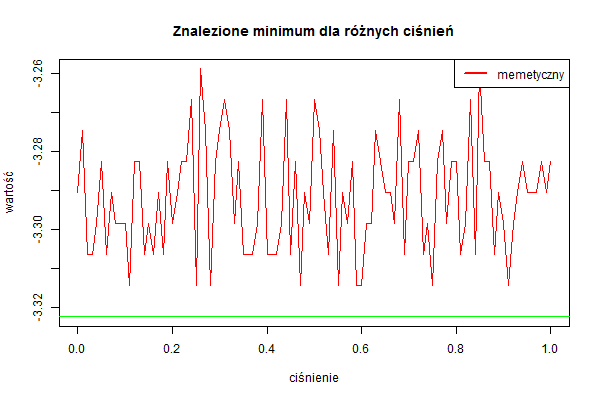
\includegraphics[width=0.95\textwidth]{./assets/Hartman6pressel.png}
	\caption{Jakość rozwiązań dla różnych wartości ciśnienia (memetyczny)}
	\label{fig:hybridpressel}
\end{figure}

\fbi
Wartości na wykresie (rys.~\ref{fig:hybridpressel}) różnią się od siebie o nie więcej niż 0,06. Oznacza to niski wpływ ciśnienia na rezultat algorytmu podobnie jak w przypadku lokalnego wyszukiwania poprzednio. Nie zauważalne są trendy w zakresie wartości wraz ze wzrostem ciśnienia. Nie można wskazać zalecanej wartości parametru na podstawie przeprowadzonego badania.

\begin{figure}[H]
	\centering
	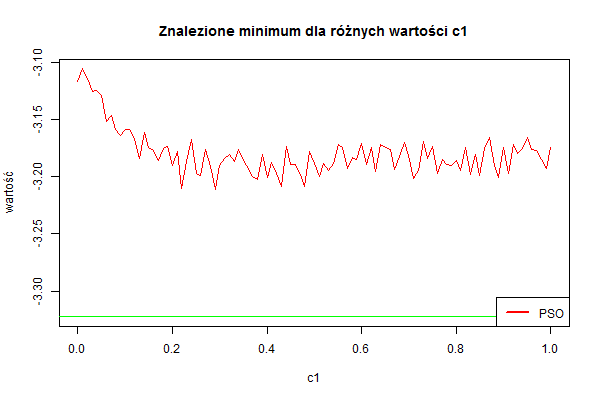
\includegraphics[width=0.95\textwidth]{./assets/Hartman6c1.png}
	\caption{Jakość rozwiązań dla różnych wartości parametru c1 algorytmu PSO}
	\label{fig:psoc1}
\end{figure}

\fbi
Z przeprowadzonych badań wynika, że najlepsze rezultaty otrzymano dla wartości c1 przekraczających 0,2. Natomiast po przekroczeniu tego umownego progu różnice wyników spowodowane są już tylko heurystyką algorytmu. Ogólnie rzecz biorąc gdyby należało wskazać zalecany parametr domyślny to byłoby to 0,2 na podstawie tych pomiarów.

\begin{figure}[H]
	\centering
	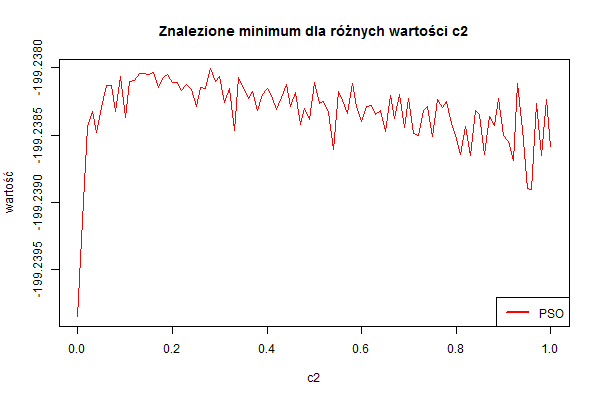
\includegraphics[width=0.95\textwidth]{./assets/Hartman6c2.png}
	\caption{Jakość rozwiązań dla różnych wartości parametru c2 algorytmu PSO}
	\label{fig:psoc2}
\end{figure}

\fbi
Tak jak w przypadku parametru c1 najlepsze rezultaty uzyskano po przekroczeniu wartości 0,2. Jednak w tym przypadku można zauważyć powolne pogorszenia się wyników wraz ze wzrostem wartości parametru c2. Zatem podobnie jak poprzednio sugerowaną wartością domyślną powinno być 0,2 -- chociaż być może tylko dla tej konkretnie badanej funkcji.

\fbi
Algorytm PSO badano dla ilości cząstek równej 500 i ilości przebiegów równej 50.

\newpage
\section{Problem komiwojażera}
\paragraph{}
Problem komiwojażera (ang. travelling salesman problem) w wersji optymalizacyjnej polega na znalezieniu minimalnego cyklu Hamiltona w pełnym grafie ważonym, który ma \textit{n} wierzchołków -- można przyjąć, że każdy wierzchołek reprezentuje miasto. Waga każdej krawędzi może oznaczać odległość pomiędzy konkretnymi miastami. Rozróżnić można wersję symetryczną (drogi z miasta A do miasta B oraz z miasta B do A mają jednakowe wagi) bądź niesymetryczną, w której odległości między miastami różnią się w zależności od punktu startowego. Problem sprowadza się do znalezienia takiej sekwencji odwiedzania miast, by każde z nich została odwiedzone tylko raz, a sumaryczna droga (a więc suma wag krawędzi) była jak najmniejsza.

\fbi
Parametrami zadania są:
\begin{itemize}
	\item skończony zbiór n-miast $ C = {c_1,c_2,…,c_n} $
	\item skończony zbiór odległości $ d_ij $, z miasta $ c_i $ do $ c_j $
	\item jeśli rozpatrujemy wersję symetryczną $ d_ij = d_ji $
	\item jeśli rozpatrujemy wersję asymetryczną, brak powyższego wymogu
\end{itemize}

\fbi
Należy określić kolejność odwiedzania wszystkich miast $ < c_{i1},c_{i2},...,c_{in} > $, aby sumaryczna trasa była jak najkrótsza, przy założeniu, że każde miasto zostało odwiedzone dokładnie jeden raz.

\begin{equation}\label{eq:tspproblem}
min (\sum_{j=1}^{n-1} d_{ij, i(j+1)} + d_{in, i1})
\end{equation}

\subsection{Przebieg i wyniki badań dla algorytmu genetycznego}
\paragraph{}
Badania z zakresu optymalizacji marszruty przeprowadzono dla symetrycznego problemu komiwojażera z wagami będącymi odległościami euklidesowymi. Wykorzystano trzy instancje z biblioteki TSPLIB:

\begin{itemize}
	\item eil51
	\item eil76
	\item eil101
\end{itemize}

\fbi
W celu porównania osiągów algorytmu pomiędzy instancjami wprowadzono metrykę jakości rozwiązań wyrażoną wzorem:

\begin{equation}\label{eq:tspquality}
quality\ of\ solution = \frac{shortest\ known \ path}{best\ found\ path} * 100\%
\end{equation}

\fbi
Wszystkie pomiary powtórzone zostały 15-krotnie celem uśrednienia. Na ilustracji (rys.~\ref{fig:tsppop}) przedstawiono wyniki dla różnych rozmiarów populacji.

\begin{figure}[H]
	\centering
	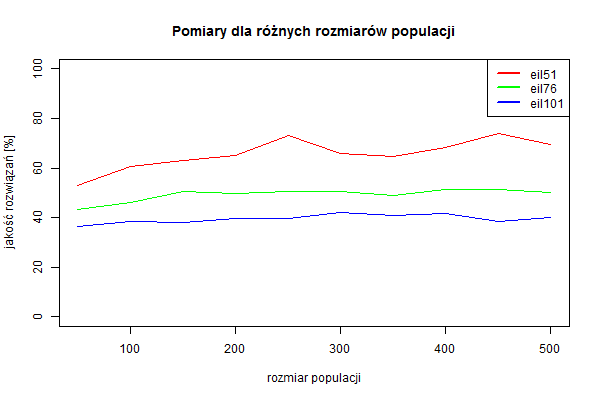
\includegraphics[width=0.9\textwidth]{./assets/tsp_pop.png}
	\caption{Jakość rozwiązań dla różnych rozmiarów populacji}
	\label{fig:tsppop}
\end{figure}

\fbi
Dla wszystkich badanych instancji zwiększenie populacji wpłynęło pozytywnie na jakość otrzymanego rozwiązania, co najbardziej obrazuje instancja ,,eli51'', która poprawiła się o~ok. 20 punktów procentowych w badanym obszarze. Natomiast ogólnie rzecz biorąc wyniki są dalekie od ideału.

\fbi
Na ilustracji (rys.~\ref{fig:tspmut}) przedstawiono wyniki pomiarów dla różnych wartości p. mutacji dla domyślnego operatora.

\begin{figure}[H]
	\centering
	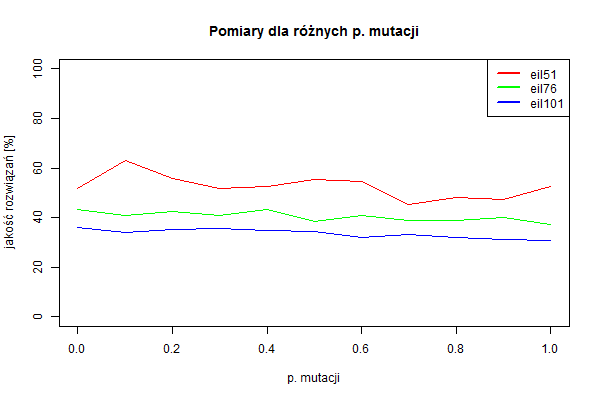
\includegraphics[width=0.9\textwidth]{./assets/tsp_mut.png}
	\caption{Jakość rozwiązań dla różnych wartości p. mutacji}
	\label{fig:tspmut}
\end{figure}

\fbi
Na podstawie powyższego wykresu nie można ustalić bezpośredniego wpływu prawdopodobieństwa mutacji na jakość rozwiązań dla instancji ,,eli76'' i ,,eli101''. Dla instancji ,,eli51'' jakość wydaje się zmniejszać wraz ze wzrostem prawdopodobieństwa mutacji. Jednakże nie są to różnice, które pozwalają na wskazanie optymalnej wartości dla omawianego parametru.

\fbi
Na ilustracji (rys.~\ref{fig:tspmutcust}) przedstawiono wyniki pomiarów dla różnych wartości p. mutacji z~niestandardowym operatorem.

\begin{figure}[H]
	\centering
	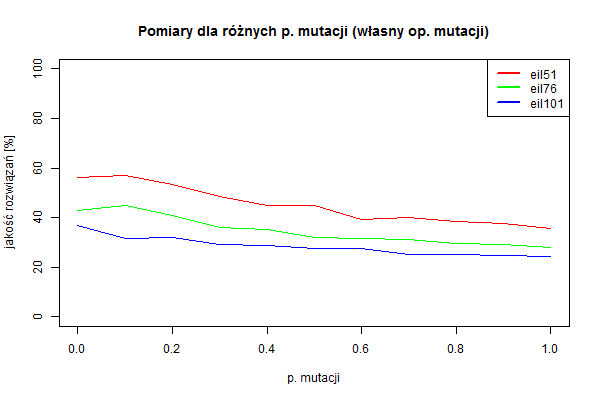
\includegraphics[width=0.9\textwidth]{./assets/tsp_mut_custom.png}
	\caption{Jakość rozwiązań dla różnych wartości p. mutacji (dla własnego operatora)}
	\label{fig:tspmutcust}
\end{figure}

\fbi
W przypadku własnej funkcji mutacji jakość rozwiązań problemu komiwojażera widocznie pogarsza u wszystkich instancji wraz ze wzrostem prawdopodobieństwa mutacji. W~przypadku ,,eli51'' jest to nawet 20 punktów procentowych.

\subsection{Słowo na temat operatora mutacji}
\paragraph{}
Operator mutacji otrzymano poprzez połączenie dostępnych w pakiecie \textit{GA} operatorów odpowiednio: insertion (losowo wybrane miasto jest usuwane i wstawiane ponownie do sekwencji w inne losowe miejsce), displacement (miasta z wybranego losowo zakresu są przemieszczane w inne miejsce bez zmiany kolejności sekwencji) oraz scramble (losowo wybierany jest zakres pomiędzy którym kolejność miast jest mieszana).

\newpage
\section{Implementacja}
\paragraph{}
Poniżej zamieszczono kody skryptów w~języku R przygotowanych w~celu umożliwienia przeprowadzenia pomiarów. Wykorzystano dwa osobne skrypty kolejno dla optymalizacji funkcji z pakietu ,,globalOptTests'' i problemu komiwojażera.

\lstinputlisting[label=lst:skryptGlowny,caption=Skrypt w~języku R wykorzystany do badań optymalizacji funkcji,firstline=1,lastline=500]{./assets/skrypt_lab35_funkcja.R}

\fbi
Skrypt przygotowano w~sposób który umożliwia w~pełni automatyczne przeprowadzenie wszystkich pomiarów. Poniżej pokrótce omówiono podstawowe parametry.


\begin{itemize}
	\item nOfRuns
	
	Ilość powtórzeń dla każdego pomiaru w~celu uśrednienia.
	
	\item colors, GAWithHybridColors, series, GAWithHybridSeries
	
	Wektory kolorów i~nazw kolejnych serii pomiarowych dla różnych rodzajów pomiarów.
	
	\item funcName
	
	Nazwa funkcji dla których przeprowadzane są pomiary.
	
	\item poptim, pressel
	
	Domyślne parametry algorytmu hybrydowego.
	
\end{itemize}

\fbi
Całość informacji niezbędnych do przeprowadzenia obliczeń odczytywana jest na podstawie nazwy funkcji z~pakietu ,,globalOptTests''. Są to: rozmiar problemu (ilość parametrów), domyślne ograniczenia, wartość w~danym punkcie oraz optimum dla domyślnych ograniczeń.

\fbi
Dodatkowo warto wspomnieć, iż algorytm ,,psoptim'' w trochę inny sposób niż genetyczny przekazuje parametry do ewaluowanej funkcji. W tym przypadku jest to macierz w której kolumny to kolejne parametry natomiast wiersze odpowiadają kolejnym cząstkom. Zatem wymagane jest by funkcja umożliwiała wektorową ewaluację parametrów. Z~uwagi na wykorzystywanie funkcji z pakietu ,,globalOptTests'' wymagało to utworzenia odpowiedniego wrappera.

\fbi
Poniżej skrypt wykorzystany dla badania algorytmu genetycznego dla problemu komiwojażera.

\lstinputlisting[label=lst:skryptKomiwojazer,caption=Skrypt w~języku R wykorzystany do badań dla problemu komiwojażera,firstline=1,lastline=500]{./assets/skrypt_lab35_komiwojazer.R}

Poniżej pokrótce omówiono podstawowe parametry.

\begin{itemize}
	\item numberOfMeasurements
	
	Ilość powtórzeń dla każdego pomiaru w~celu uśrednienia.
	
	\item instances
	
	Instancje problemu TSP, dla których przeprowadzane są testy.
	
	\item best\_solutions
	
	Wektor zawierający optymalne rozwiązania dla instancji.
	
	\item colors
	
	Kolory dla wykresu.
	
\end{itemize}

\newpage
\section{Podsumowanie}
\paragraph{}
W trakcie przeprowadzonych badań przetestowano algorytmy w wariantach: genetyczny domyślny, genetyczny z własną funkcją mutacji, hybrydowy domyślny oraz hybrydowy z własną funkcją mutacji a także algorytm optymalizacji rojem cząstek -- dla problemu optymalizacji rzeczywistej. Przeprowadzono także testy dla algorytmu genetycznego (domyślnego jak również ze zmodyfikowaną funkcją mutacji) dla problemu TSP.

\fbi
Zmiana funkcji mutacji dla optymalizacji rzeczywistej nie spowodowała znaczących różnic w jakości otrzymywanych rozwiązań. Jej działanie okazało się porównywalne z zaimplementowaną funkcją. W przypadku problemu TSP przygotowana funkcja mutacji będąca złożeniem kilku domyślnych funkcji mutacji okazała się gorsza od domyślnej (pogorszyła rezultaty o ok. 10 punktów procentowych).

\fbi
Z przeprowadzonych badań wynika brak lub niski wpływ dokonanych modyfikacji funkcji mutacji na działanie badanych algorytmów. Warto wspomnieć, że również w samym pakiecie GA jest możliwość wyboru spośród kilku dostępnych funkcji mutacji i krzyżowania.

\fbi
Algorytm memetyczny umożliwia uzyskanie rezultatów porównywalnych ze zwykłym genetycznym. Różnice zaobserwowane podczas badań są niewielkie i~nie można jednoznacznie rozstrzygnąć na ich podstawie. Szczególnie zważywszy na fakt, że tylko pewna część parametrów podlegała badaniu. Patrząc jednak na oba algorytmy z perspektywy przeglądu statycznego -- algorytm memetyczny z~zasady pozwala uzyskać lepsze wyniki z~uwagi na dodatkowe ,,polerowanie'' wyniku w okolicy znalezionego przez algorytm genetyczny optimum.

\fbi
Algorytm PSO dla przyjętych parametrów domyślnych okazał się gorszy niż badane poprzednio.

\newpage
\begin{thebibliography}{40}

\bibitem{test1}
Artur Suchwałko ,,Wprowadzenie do R dla programistów innych języków'' https://cran.r-project.org/doc/contrib/R-dla-programistow-innych-jezykow.pdf

\bibitem{test2}
Luca Scrucca ,,Package GA''
https://cran.r-project.org/web/packages/GA/GA.pdf

\bibitem{test3}
Surjanovic, S. \& Bingham, D. (2013). ,,Virtual Library of Simulation Experiments: Test Functions and Datasets.'' Retrieved April 3, 2017, from http://www.sfu.ca/~ssurjano.

\bibitem{test4}
Momin Jamil, Xin-She Yang ,,A literature survey of benchmark functions for global optimization problems'', Int. Journal of Mathematical Modelling and Numerical Optimisation, Vol. 4, No. 2, pp. 150–194. (2013)

\bibitem{test5}
Ajith Abraham, Aboul-Ella Hassanien, Patrick Siarry, Andries Engelbrecht, ,,Foundations of Computational Intelligence Volume 3'' (2009)

\bibitem{test6}
Onay Urfalioglu, Orhan Arikan ,,Self-adaptive randomized and rank-based differential evolution for multimodal problems'' (2011)

\end{thebibliography}

\end{document}